\documentclass[a4paper, oneside, 11pt]{article}
%% -> Für längere Arbeiten "report" benutzen.

%% --------------------------------------------------------------------- %%
\usepackage{pdfpages}
\usepackage{ifthen}
\newboolean{english}
%\setboolean{english}{true} %% -> Kommentar entfernen bei englischen Arbeiten

%% --------------------------------------------------------------------- %%

%% -> Einfügen der Definitionen
%% -> Deutsche Anpassung 
\usepackage[T1]{fontenc}
\usepackage[ngerman,english]{babel}
%\usepackage{babelbib}
\usepackage{ifthen}
%% --------------------------------------------------------------------- %%

%% -> Farben einfügen
\usepackage{color}
\usepackage{xcolor}

% -> Definierte Farben
\definecolor{MSBlue}{rgb}{.204,.353,.541} 
\definecolor{trueblue}{rgb}{0.0, 0.45, 0.81}
\definecolor{onyx}{rgb}{0.06, 0.06, 0.06}
\definecolor{mygruen}{rgb}{0.4660, 0.6740, 0.1880}
\definecolor{plotblue}{rgb}{0, 0.4470, 0.7410}
\definecolor{myrot}{rgb}{0.8500, 0.3250, 0.0980}
\definecolor{mygreen}{RGB}{28,172,0} %% Matlab Kommentar
\definecolor{mylilas}{RGB}{170,55,241} %% Matlab String

%% --------------------------------------------------------------------- %%

%% -> Grafiken 
\usepackage{graphicx}
\usepackage{epstopdf}
\usepackage{wallpaper}
\usepackage{float} %% Verbessert die Platzierung
\usepackage{placeins} %Für \FloatBarrier beim Einfügen von Abbildungen
\usepackage{matlab-prettifier} % MATLAB code
\usepackage{epstopdf}
%% --------------------------------------------------------------------- %%

\usepackage[tmargin=1in,bmargin=1in,lmargin=1.25in,rmargin=1.25in]{geometry}
\setlength{\parindent}{0em}
\setlength{\parskip}{1.5ex plus0.5ex minus0.5ex}
\usepackage{setspace}
\onehalfspacing

\usepackage{pst-all} %% erweiterte Zeichenbefehle

%% -> Schriftart
\usepackage{helvet}
\renewcommand{\familydefault}{phv}

%% -> Layout Überprüfung
\usepackage{layout}
\usepackage{xspace}

%% -> Für Tabellen
\usepackage{array}
\usepackage{booktabs}
\usepackage{dcolumn}
\usepackage{multirow}

%% -> Einrücken von und Abstand zwischen Absätzen
\setlength{\parindent}{0em}
\setlength{\parskip}{1.5ex plus0.5ex minus0.5ex}

%% -> Tabulator Funktion
\newcommand\tab[1][1cm]{\hspace*{#1}}

%% -> Weniger Warnungen wegen überfüllter Boxen
\tolerance = 9999
\sloppy

%% -> Erweiterte Einstellungen der Bildunterschriften bzw. Tabellenunterschriften
\usepackage{caption}
\usepackage{subcaption}
\captionsetup[figure]{labelfont=footnotesize, textfont=footnotesize}
%\captionsetup[table]{labelfont=footnotesize, textfont=footnotesize}

%% -> Hyperref
%\usepackage[pdftex,bookmarks=true,bookmarksnumbered=true,]{hyperref}

\usepackage[hidelinks]{hyperref}
% \usepackage[colorlinks=true]{hyperref}
% \hypersetup{
% colorlinks=true,
% linkbordercolor={1 0 0},
% citebordercolor={0 1 0},
% filebordercolor={1 0 1},
% runbordercolor={1 0 1},
% urlbordercolor={0 0 1},
% }

%% -> Quellen
\usepackage[super, square, sort&compress]{natbib}

%%-> Weitere nützliche Pakete
\usepackage{todonotes}
\setlength {\marginparwidth }{2cm}
%% --------------------------------------------------------------------- %%

% -> Für Codes zum einfügen
\usepackage{listings}
%\lstset{numbers=left,numberstyle=\tiny,stepnumber=5,numbersep=5pt}

%% -> Für MATLAB Code
\lstset
{language=Matlab,%
    basicstyle=\scriptsize,
    breaklines=true,%
    captionpos=b,
    frame = single,
    morekeywords={matlab2tikz},
    keywordstyle=\color{blue},%
    morekeywords=[2]{1}, keywordstyle=[2]{\color{black}},
    identifierstyle=\color{black},%
    stringstyle=\color{mylilas},
    commentstyle=\color{mygreen},%
    showstringspaces=false,%
    %numbers=left,%
    %numberstyle={\footnotesize \color{black}},%
    %stepnumber=5, %
    %numbersep=9pt, % 
    emph=[1]{for,end,break},emphstyle=[1]\color{red}, %
    emph=[2]{all}, emphstyle=[2]\color{mylilas},    
}
%% --------------------------------------------------------------------- %%

% -> Kopf und Fußzeile gestallten
\usepackage{fancyhdr}
\setlength{\headheight}{13.6pt}
\setlength{\footskip}{41pt}
\rhead{} 
\chead{} 
\lhead{}
\renewcommand{\headrulewidth}{0pt}
\lfoot{\includegraphics[width=\textwidth*1/6]{Definition/DUH-positive.eps}}
\rfoot{\small\thepage}
\cfoot{}
\renewcommand{\footrulewidth}{0pt}
%% --------------------------------------------------------------------- %%

%% -> Matematische Packages
\usepackage{amsmath,amssymb,amsfonts,amstext}
\usepackage{mathtools}
\usepackage{mathrsfs}

%% -> SI-Einheiten
%\usepackage{units}
\usepackage{siunitx}
% \usepackage{physics}
\sisetup{locale = DE,separate-uncertainty}
\sisetup{list-final-separator={ und }}
\sisetup{per-mode=fraction}
\DeclareSIUnit\Pascal{\newton\per\square\metre}
%\sisetup{output-decimal-marker = {.}} %% Für Punkttrennung nur bei englischen Arbeiten erforderlich
%% --------------------------------------------------------------------- %%

%% -> Für die Überschriften
\usepackage{titlesec}
\titleformat{\section}{\LARGE\sffamily\bfseries}{\thesection}{1em}{}
\titleformat{\subsection}{\Large\bfseries\sffamily}{\thesubsection}{1em}{}
\titleformat{\subsubsection}{\large\sffamily\bfseries}{\thesubsubsection}{1em}{}
%% --------------------------------------------------------------------- %%

%% -> Bildnummerierung ist logisch mit Kapitelnummerierung
\numberwithin{figure}{section}
\numberwithin{table}{section}
\numberwithin{equation}{section}
%\numberwithin{equation}{subsection}
%% --------------------------------------------------------------------- %%

%% -> Schaltplan zeichnen und Grafiken und für PGF Plots
\usepackage[european, siunitx]{circuitikz}
\usetikzlibrary{circuits.ee.IEC}
\usepackage{tikz}
\usepackage{tikzscale}
\usepackage{pgfplots}
\pgfplotsset{compat=1.4}
\newlength\figH
\newlength\figW
\setlength{\figH}{6cm}
\setlength{\figW}{8cm}
%% --------------------------------------------------------------------- %%

%% -> Für Vektoren
\usepackage{amsmath}

% For pie-charts
\usepackage{amsmath,amssymb,amsfonts,amstext}
\usepackage{mathtools}
\usepackage{mathrsfs}
\usepackage{pgf-pie}

%% -> Deckblatt ausfüllen 
\def\labtitle{Industrial Electronics }
\def\labcode{MECH-M-3-IEL-IEL-ILV}
\def\labname{}
\def\labnum{Berichtnummer}
\def\study{Master Mechatronic \& Smart Technologies}
\def\branch{}
\def\term{3.}
\def\lecturer{Thomas Gadner}
\def\group{MA-MECH-23-BB}
\def\student{Lukas Sieß}

%% --------------------------------------------------------------------- %%
\begin{document}
\newcounter{romanPagenumber}

%% -> Sprache auswählen
\ifthenelse{\boolean{english}}{\selectlanguage{english}}{\selectlanguage{ngerman}}
\selectlanguage{ngerman}
%\selectlanguage{english}

\pagestyle{fancy} % Fußzeile und Kopfzeile einfügen

\pagenumbering{Roman}

%% Deckblatt %%

\thispagestyle{empty}
\sffamily
\ThisTileWallPaper{\paperwidth}{\paperheight}{Deckblatt/MCIHintergrundKPL.pdf}

\vspace*{1cm}
\def\thesis{\ifthenelse{\boolean{english}}{Abschlussbericht}{Zusammenfassung}}
\textcolor{MSBlue}{\rmfamily\bfseries\Huge\thesis}

\vspace*{0.5cm}
\textbf{\labtitle{}( \labcode)}

\textbf{\labname}

%\ifthenelse{\boolean{english}}{\textbf{Report} }{\textbf{Labor }}\textbf{\labnum}


\vspace*{14cm}

\textcolor{gray}{\study}

% \def\studybranch{\ifthenelse{\boolean{english}}{Study Branch}{Studienzweig}}
% \textcolor{gray}{\studybranch: \branch}

\def\termname{\ifthenelse{\boolean{english}}{semester}{Semester}}
\textcolor{gray}{\term{ }\termname}

\def\lecturername{\ifthenelse{\boolean{english}}{Responsible lecturer}{Lehrveranstaltungsleiter}}
\textcolor{gray}{\lecturername: \lecturer}

\def\groupname{\ifthenelse{\boolean{english}}{Group}{Jahrgang}}
\textcolor{gray}{\groupname: \group}

\def\authorname{\ifthenelse{\boolean{english}}{Author}{Verfasser}}
\textcolor{gray}{\authorname: \student}

\textcolor{gray}{\today}

\newpage % Deckblatt laden

\setcounter{romanPagenumber}{\value{page}}

\tableofcontents%\thispagestyle{empty}   % Inhaltsverzeichnis
\clearpage

\pagestyle{fancy}
\pagenumbering{arabic}
% =============================================================================
\section{Einleitung} \label{sec:einleitung}

Dieser Bericht dokumentiert die Umsetzung der zweiten Aufgabe im Bereich Regelungstechnik und Leistungselektronik. Ziel ist die praxisnahe Anwendung der theoretischen Grundlagen aus den ersten beiden Semestern, indem ein Leistungselektroniksystem modelliert und geregelt wird. Dazu wird ein digitaler Regler entworfen und auf einer geeigneten Plattform implementiert.

Die Aufgabenstellung gliedert sich in zwei wesentliche Arbeitsschritte:
\begin{itemize}
    \item \textbf{Modellierung eines Leistungselektronik-Wandlers in PLECS:}
    Zunächst wird ein Modell eines Leistungselektronik-Wandlers mit PLECS erstellt. Dieses Modell bildet die Basis für die spätere Regelung. Um die Komplexität der Regelung zu minimieren, wird das System so ausgelegt, dass die Dynamik möglichst träge ist. Dadurch kann eine Regelung mit klassischen kontinuierlichen Methoden erfolgen, sofern die Abtastrate hoch genug gewählt wird.  (Siehe Abbildung: \label{fig:Soft})

    \item \textbf{Implementierung des Modells auf einer RTBox mit einem STM-Mikrocontroller als Regler:}
    Nach der Modellierung wird das System auf einer RTBox implementiert. Die Regelung erfolgt über einen STM-Mikrocontroller, der die Steueralgorithmen ausführt und das Systemverhalten in Echtzeit überprüft.
\end{itemize}

Dieser Bericht legt den Fokus auf die präzise Modellbildung, die Auswahl geeigneter Regelparameter und die Implementierung auf der RTBox mit einem STM-Mikrocontroller.
\newpage
\section{Task 1} \label{sec:Task1}


\begin{figure}[H]
    \centering
    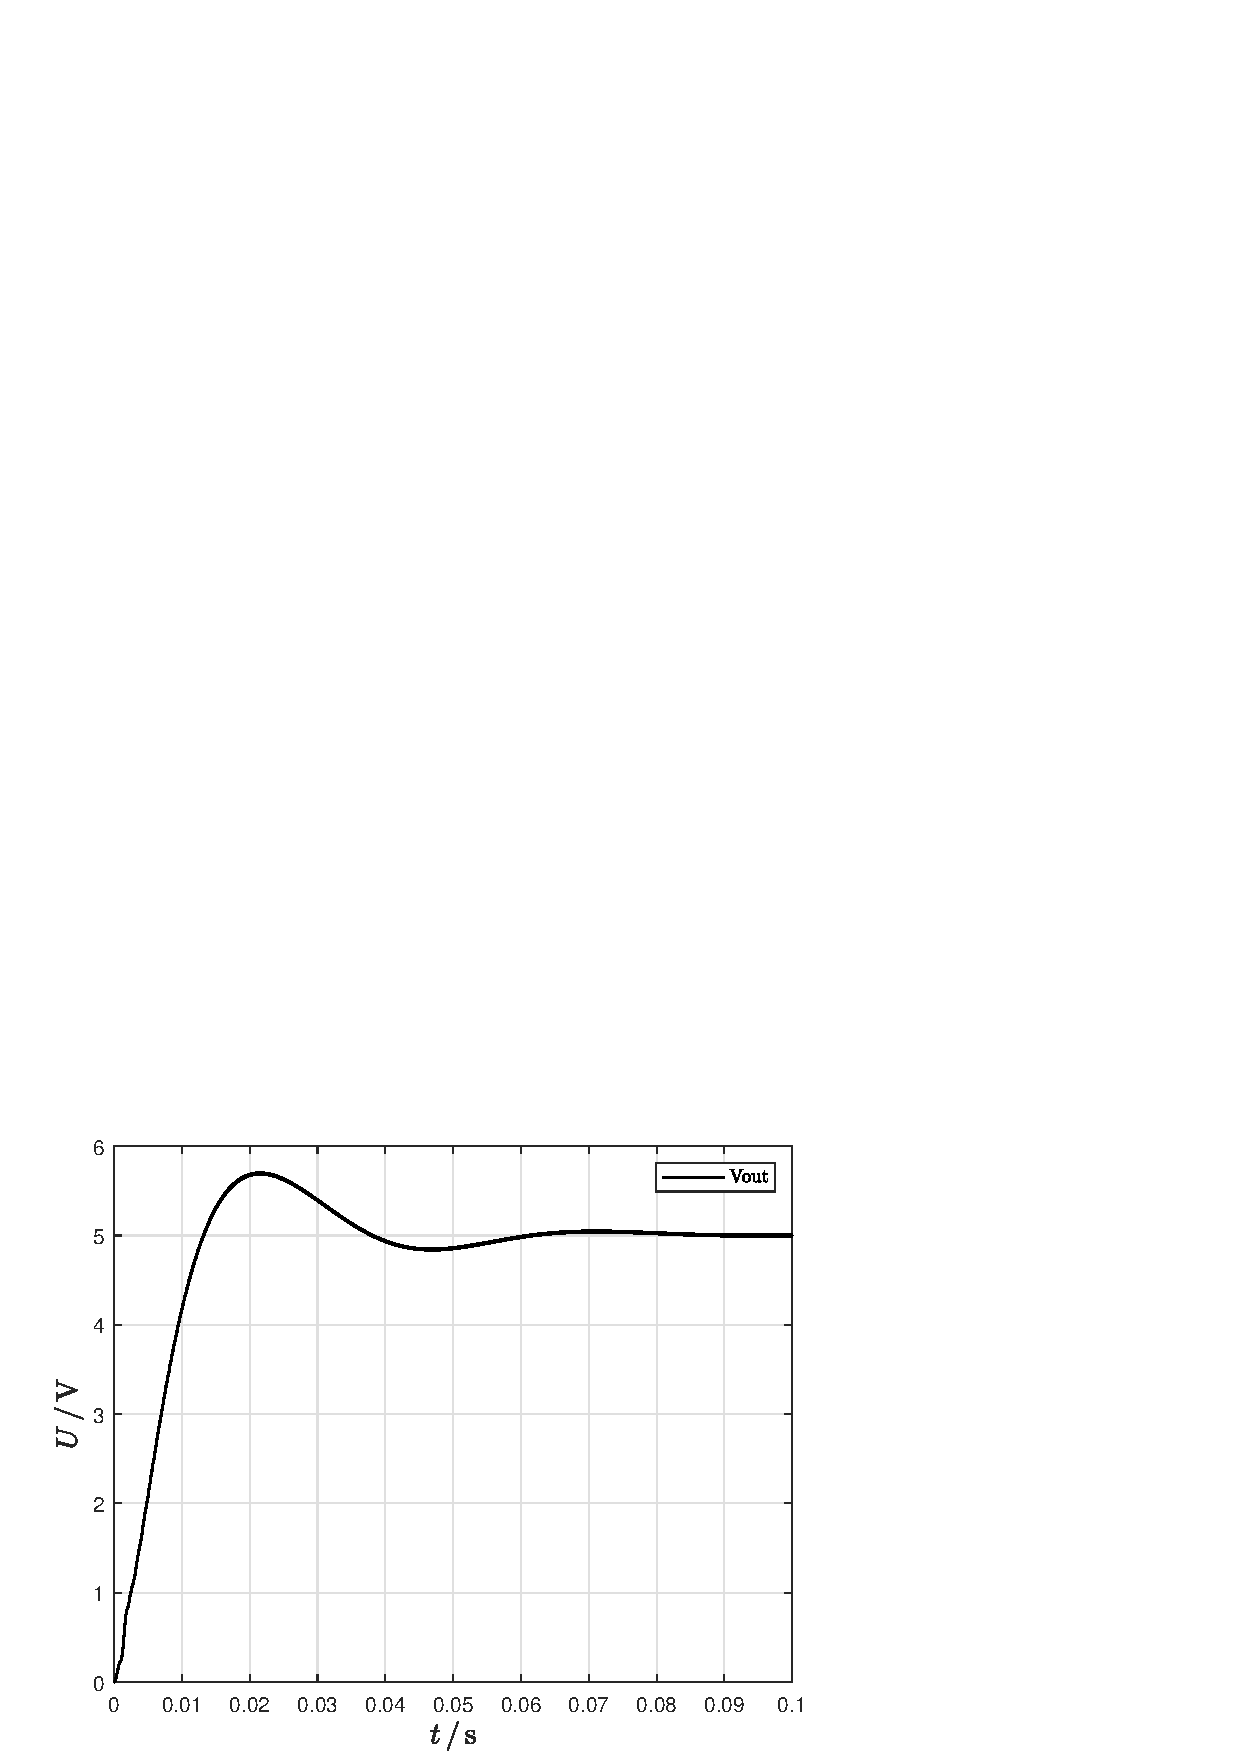
\includegraphics[width=0.8\linewidth]{Figure/Soft.png}
    \caption{FFT LTC3639 mit Filter}
    \label{fig:Soft}
\end{figure}

\begin{figure}[H]
    \centering
    \includegraphics[width=0.8\linewidth]{Figure/ControllerSoft.png}
    \caption{FFT LTC3639 mit Filter}
    \label{fig:ControllerSoft}
\end{figure}

\begin{figure}[H]
    \centering
    \includegraphics[width=0.8\linewidth]{Figure/SystemSoft.png}
    \caption{FFT LTC3639 mit Filter}
    \label{fig:SystemSoft}
\end{figure}


\subsection{PID Auslegung}

\begin{figure}[H]
    \centering
    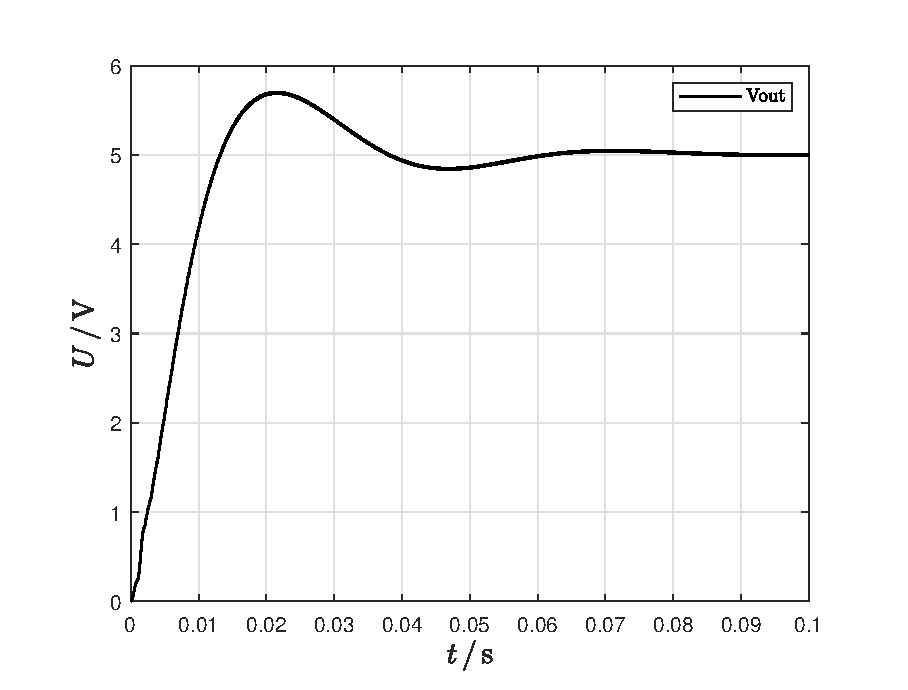
\includegraphics[width=0.8\linewidth]{Figure/Soft.eps}
    \caption{FFT LTC3639 mit Filter}
    \label{fig:SystemSoft}
\end{figure}
\newpage
\section{Task 2} \label{sec:Task2}

Nach der erfolgreichen Modellierung in PLECS wurde die Hardware-Implementierung vorbereitet. In diesem Kapitel werden die notwendigen Schritte zur Umsetzung erläutert. Dabei stehen die Echtzeitfähigkeit der RTBox, die Anbindung des Mikrocontrollers sowie die Entwicklung der Steueralgorithmen im Fokus. Die Herausforderungen der Echtzeitregelung und die erforderlichen Anpassungen werden ebenfalls behandelt. Abschließend erfolgt eine Analyse der Performance basierend auf Simulationen und experimentellen Ergebnissen.

Zur Umsetzung wurden zwei Subsysteme definiert – eines für den Controller, eines für das geregelte System. Diese Trennung ermöglicht eine separate Parametrierung der Coder-Optionen für eine optimierte Code-Generierung. Die Ein- und Ausgänge wurden wie folgt konfiguriert und miteinander verschaltet:

\begin{itemize}
    \item \textbf{System-Subsystem:} Enthält PLECS PWM Capture sowie PLECS Analog Out für Strom- und Spannungsmessung (Siehe Abbildung: Model_Task2_System.png)
 
    \item \textbf{Controller-Subsystem:} Enthält STM PWM Out für die Ansteuerung sowie STM ADC (Analog In Triggered) zur Erfassung der Systemrückmeldung. Ein Control Trigger Block wurde integriert, um den ADC korrekt zu triggern. (Siehe Abbildung: Model_Task2_Controller.png)
\end{itemize}

Die Simulation wurde mit zwei verschiedenen Lasten ($R_{Load}=\SI{2}{\ohm}$ und $R_{Load}=\SI{4}{\ohm}$) durchgeführt, um die Performance des Reglers unter verschiedenen Bedingungen zu bewerten. Das PLECS-Modell wurde schrittweise für die Hardware-Simulation mit der RTBox und dem STM32 Nucleo vorbereitet. Die in den Coder-Optionen gesetzten Parameter:

\begin{itemize}
    \item \textbf{Controller:} Target = STM32G4x; Scheduling Step Size = (Siehe Abbildung: Settings CoderOptions_Model_Task2_ControllerTarget.png)

    \item \textbf{System:} Target = PLECS RT Box 2; Scheduling Step Size =  (Siehe Abbildung: Settings CoderOptions_Model_Task2_SystemTarget.png)

    \item \textbf{Gesamtsystem-Ansicht:} Überblick der vollständigen Implementierung (Siehe Abbildung: Model_Task2.png)
\end{itemize}

\begin{figure}[H]
    \centering
    \includegraphics[width=0.6\linewidth]{Figure/Hard.png}
    \caption{FFT LTC3639 mit Filter}
    \label{fig:Hard}
\end{figure}

\begin{figure}[H]
    \centering
    \includegraphics[width=0.6\linewidth]{Figure/SystemHard.png}
    \caption{FFT LTC3639 mit Filter}
    \label{fig:SystemHard}
\end{figure}

\begin{figure}[H]
    \centering
    \includegraphics[width=0.6\linewidth]{Figure/ControllerHard.png}
    \caption{FFT LTC3639 mit Filter}
    \label{fig:ControllerHard}
\end{figure}





\subsection{Ergebnisse der Simulation an der Hardware}

Für die Evaluierung des Reglers wurden Simulationen mit zwei Lastwiderständen durchgeführt:

\begin{itemize}
    \item \textbf{Ergebnisse für $R_{Load}=\SI{2}{\ohm}$:} Die Simulation zeigt eine stabile Regelung mit geringer Überschwingung. Der Spannungsverlauf erreicht schnell den gewünschten Wert und bleibt stabil. (Siehe Abbildung: \ref{fig:Rload2})
    \item \textbf{Ergebnisse für $R_{Load}=\SI{4}{\ohm}$:} Auch bei einer höheren Last bleibt das System stabil. Die Regelung reagiert schnell und hält die Ausgangsspannung zuverlässig. Die Reaktionszeit ist etwas kürzer als bei $R_{Load}=\SI{2}{\ohm}$, was an der veränderten Systemdynamik liegt. (Siehe Abbildung: \ref{fig:Rload4})
\end{itemize}

\begin{figure}[H]
    \centering
    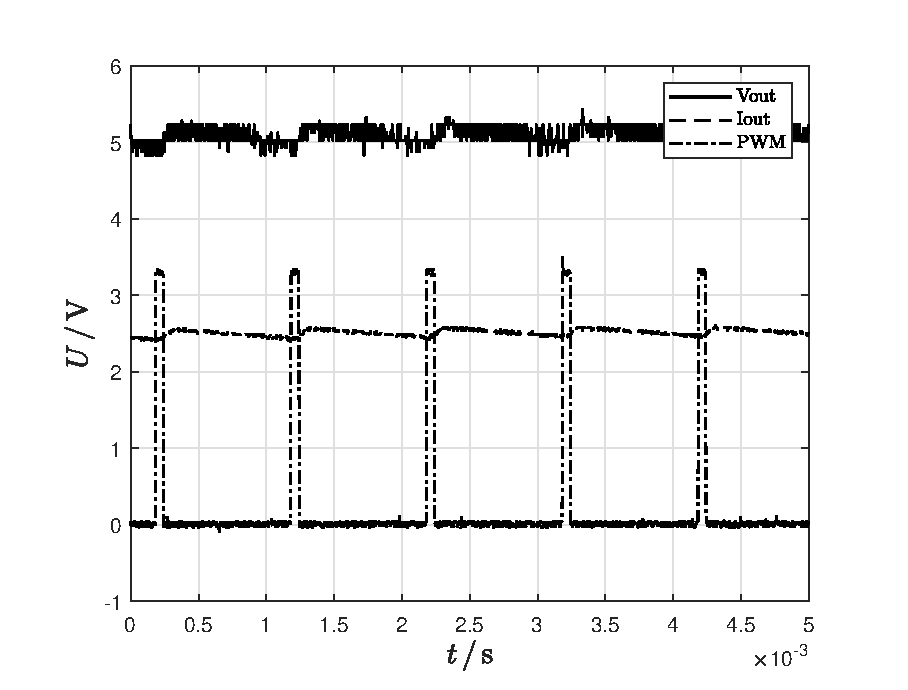
\includegraphics[width=0.6\linewidth]{Figure/Rload2.eps}
    \caption{Messung mit $R_{load} = \SI{2}{\ohm}$}
    \label{fig:Rload2}
\end{figure}

\begin{figure}[H]
    \centering
    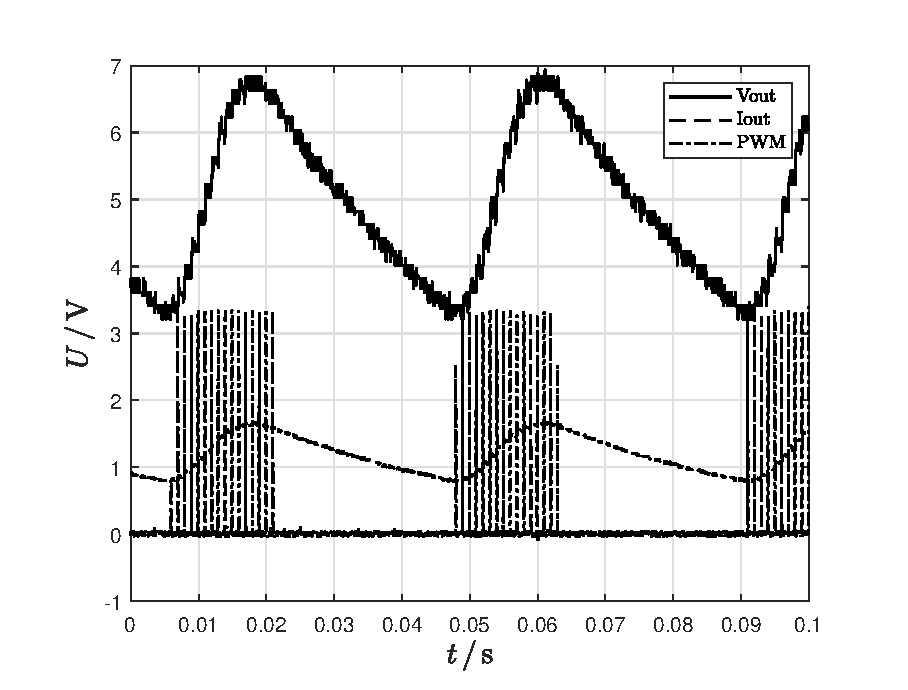
\includegraphics[width=0.6\linewidth]{Figure/Rload4.eps}
    \caption{Messung mit $R_{load} = \SI{4}{\ohm}$}
    \label{fig:Rload4}
\end{figure}
\newpage
\section{Layout-Empfehlungen für das Board-Design}\label{sec:Layout}

Für ein EMV-konformes Design mit dem LTC3639 sollten folgende Punkte beachtet werden:

\begin{enumerate}
    \item \textbf{Kondensatoren nahe den Pins des LTC3639} platzieren, um parasitäre Induktivitäten und Widerstände zu minimieren.
    \item \textbf{Masseverbindungen} durch ein durchgehendes Masse-Plane sicherstellen, um Rauschen und Spannungsdifferenzen zu reduzieren.
    \item \textbf{Schleifenflächen minimieren}, um elektromagnetische Störungen zu verringern.
    \item \textbf{Hochfrequenz- und Niedrigfrequenzkomponenten} räumlich oder auf verschiedenen Plane-Ebenen trennen.
    \item \textbf{Thermisches Management} durch ausreichende Kühlflächen für Wärmequellen wie den LTC3639.
    \item \textbf{Filterkomponenten} nah an den Regleranschlüssen platzieren, um leitungsgebundene Störungen zu dämpfen.
    \item \textbf{Signalpfade kurz halten} und unnötige Kreuzungen zwischen Hoch- und Niedrigfrequenzleitungen vermeiden.
    \item \textbf{Stromversorgungsleitungen} breit und direkt führen, um Spannungsabfälle und Erwärmung zu minimieren.
\end{enumerate}

Diese Maßnahmen verbessern die EMV-Leistung und die Zuverlässigkeit des Designs.


\newpage
% =============================================================================

\clearpage

%% -> Verzeichnisse
\pagestyle{fancy}
\pagenumbering{Roman}
\addtocounter{romanPagenumber}{1}
\setcounter{page}{\theromanPagenumber}
%% --------------------------------------------------------------------- %%
\clearpage
%Appendix
\clearpage
\fancyhead[L]{}
\fancyhead[R]{\MakeUppercase{ANHANG}}
\appendix 
\addcontentsline{toc}{section}{ANHANG}
\section{Anhang}\label{app:1}

\subsection{MATLAB Skript}\label{a1:matlab} 

\end{document}
